\documentclass[12pt]{article}
\usepackage[utf8]{inputenc}
\usepackage[T1]{fontenc}
\usepackage{amsmath,amssymb}
\usepackage{booktabs}
\usepackage{graphicx}
\usepackage[margin=1in]{geometry}
\usepackage{setspace}
\usepackage{natbib}
\usepackage{hyperref}
\usepackage{float}

\doublespacing
\bibliographystyle{aer}

\title{Commodity Busts and the Selective Erosion of Civil Liberties:\\Evidence from an Asymmetric Event Study}
\author{Working Paper --- Revised}
\date{\today}

\begin{document}
\maketitle

\begin{abstract}
Do commodity price busts permanently erode civil liberties? Using an asymmetric event study on 80 commodity-dependent countries over 1975--2018, I exploit exogenous variation from the IMF's Commodity Terms of Trade index to estimate the heterogeneous and dynamic effects of commodity busts across five civil liberty dimensions. Fair trial rights are the only liberty significantly affected by busts in the TWFE specification ($\beta = -0.199$, $p = 0.020$), a finding robust to alternative bust thresholds and to exclusion of the COVID-19 period ($p = 0.063$). The event-study dynamics reveal that bust and recovery effects are statistically asymmetric for four of five liberties ($p < 0.001$), but this asymmetry reflects heterogeneous \textit{improvement} trajectories rather than a simple ratchet pattern. Freedom of movement initially appeared to exhibit a ratchet, but this result does not survive exclusion of COVID-era movement restrictions or placebo timing tests ($p = 0.926$). Pre-trend tests support parallel trends for all five liberties ($F$-test $p > 0.19$). The results demonstrate that commodity shocks selectively target judicial institutions while leaving other civil liberties largely unaffected, consistent with executive strategies that prioritize weakening the institutional constraints on their power.

\medskip
\noindent\textbf{JEL Codes:} D72, O13, P16, Q33 \\
\textbf{Keywords:} commodity shocks, civil liberties, democratic backsliding, asymmetric event study, fair trial
\end{abstract}

\newpage

\section{Introduction}

The resource curse literature has extensively documented the relationship between commodity wealth and political outcomes \citep{ross2015, tsui2011, aslaksen2010}. Yet this literature overwhelmingly treats political outcomes as unidimensional, asking whether shocks make countries ``more'' or ``less'' democratic. This framing obscures a critical question: \textit{which specific civil liberties} are most vulnerable to commodity busts?

This paper makes two contributions. First, I disaggregate political outcomes into five distinct civil liberty dimensions---freedom of expression, assembly, religion, movement, and fair trial---using the Civil Liberty Dataset \citep{coppedge2023}. Second, I test for asymmetry in the dynamic response by comparing bust-period dynamics against recovery-period dynamics using separate event studies.

The identification strategy exploits the Commodity Terms of Trade (CTOT) index \citep{grussKebhaj2019}, which weights world commodity prices by each country's fixed export-import commodity basket, providing plausibly exogenous variation. I define bust episodes as cumulative three-year CTOT declines exceeding 20\%, yielding 31 bust and 21 recovery episodes across 80 countries.

The central finding is that commodity busts \textit{selectively} target fair trial rights ($\beta = -0.199$, $p = 0.020$) while leaving the other four liberties statistically unaffected. This result is robust to alternative bust thresholds ($-15\%$, $-25\%$, $-30\%$) and survives exclusion of the COVID-19 period ($p = 0.063$). The event-study symmetry tests reveal statistically significant asymmetry between bust and recovery dynamics for four of five liberties, but careful examination shows this reflects heterogeneous improvement patterns, not a simple ``ratchet'' of deterioration without recovery. An initial finding of a ratchet effect for freedom of movement does not survive COVID-era exclusion or placebo timing tests, underscoring the importance of confounder scrutiny.

These findings contribute to the democratic backsliding literature \citep{bermeo2016} by identifying judicial institutions as the specific channel through which commodity crises erode democratic governance, and to the resource curse literature \citep{ross2015} by demonstrating that the political costs of commodity dependence are concentrated in a single institutional dimension rather than distributed across all civil liberties.

\section{Literature Review}

\subsection{Commodity Shocks and Political Outcomes}

\citet{tsui2011} shows that oil discoveries reduce subsequent democratization, while \citet{dubeVargas2013} demonstrate that commodity price shocks affect civil conflict intensity in Colombia. \citet{bruckner2010} provide cross-country evidence linking negative commodity price shocks to conflict onset in Sub-Saharan Africa. \citet{bazziBlattman2014} offer a more nuanced view, finding that the commodity--conflict relationship depends on the type of commodity and the institutional context. \citet{ross2015} surveys this literature and concludes that the resource curse operates primarily through institutional channels.

\subsection{Democratic Backsliding}

\citet{bermeo2016} argues that modern democratic erosion occurs through selective institutional degradation rather than outright regime change. \citet{levitskyWay2010} document how competitive authoritarian regimes strategically restrict specific political rights while maintaining electoral facades. This literature motivates the disaggregated approach pursued here: if backsliding is selective, aggregate democracy indices will understate the damage to specific institutions.

\section{Data}

\subsection{Civil Liberty Dataset}

The outcome variables come from the Civil Liberty Dataset v2.10, providing ordinal measures (1--4 scale) of five civil liberties for 204 countries from 1975 to 2025 \citep{coppedge2023}. Following referee guidance, the primary estimation sample is restricted to 1975--2018 to avoid confounding from COVID-19 emergency restrictions, which disproportionately affected freedom of movement.

\subsection{Commodity Terms of Trade}

The CTOT index \citep{grussKebhaj2019} provides country-specific commodity price indices for 180 countries from 1962 to 2024. The index weights world commodity prices by each country's export-import commodity basket using fixed trade shares, ensuring variation is driven by global price movements.

\subsection{Merged Sample and Episode Identification}

Merging CLD and CTOT yields 7,330 country-year observations covering 80 commodity-dependent countries. Bust episodes are defined as cumulative three-year CTOT declines exceeding $-20\%$ (31 episodes); recovery episodes as subsequent increases exceeding $+20\%$ (21 episodes).

\begin{table}[htbp]
\centering
\caption{Summary Statistics}
\label{tab:summary}
\begin{tabular}{lccccc}
\toprule
Variable & Mean & SD & Min & Max & N \\
\midrule
  Expression & 2.57 & 0.93 & 1.0 & 4.0 & 7,330 \\
  Assembly & 2.81 & 1.07 & 1.0 & 4.0 & 7,330 \\
  Religion & 3.27 & 0.83 & 1.0 & 4.0 & 7,330 \\
  Movement & 3.16 & 0.82 & 1.0 & 4.0 & 7,330 \\
  Fair Trial & 2.26 & 0.95 & 1.0 & 4.0 & 6,824 \\
  Ctot Index & 95.71 & 9.37 & 38.3 & 162.9 & 7,330 \\
  Ctot Pct Change & 0.17 & 5.00 & -41.4 & 72.0 & 7,250 \\
\bottomrule
\end{tabular}
\end{table}

\section{Empirical Strategy}

\subsection{TWFE Specification}

The baseline specification estimates the average bust effect on each liberty:
\begin{equation}
\text{Liberty}_{it} = \alpha_i + \gamma_t + \beta \cdot \text{Bust}_{it} + \varepsilon_{it}
\end{equation}
with country and year fixed effects and standard errors clustered at the country level ($N = 80$). This specification captures the average within-country, within-year effect of being in a bust episode.

\textit{Note on staggered timing:} The 31 bust episodes have heterogeneous timing. In the presence of treatment effect heterogeneity, TWFE estimates may be biased \citep{goodmanBacon2021}. However, bust episodes are transitory (average duration 3--4 years), not absorbing treatments, which mitigates the negative-weighting concern that motivates Callaway-Sant'Anna or Sun-Abraham estimators. These estimators are designed for permanent, staggered treatment adoption. I report the event study dynamics as a complement that reveals time-varying effects without imposing the constant-effect restriction of TWFE.

\subsection{Asymmetric Event Study}

Separate event studies are estimated for bust and recovery episodes (reference period $k = -1$, window $k \in [-3, +5]$). The symmetry test evaluates:
\begin{equation}
H_0: \bar{\beta}^{\text{bust}}_{\text{post}} + \bar{\beta}^{\text{recovery}}_{\text{post}} = 0
\end{equation}

\textit{Reconciling TWFE and event-study magnitudes:} The TWFE estimate uses the full panel with the bust dummy, while the event study is estimated on the subset of countries that experienced at least one bust episode, using relative-time dummies. Differences in sample composition and the reference-period normalization ($t = -1$) mean that TWFE and event-study averages need not have identical signs. The TWFE coefficient is the preferred causal estimate; the event study reveals dynamics.

\section{Results}

\subsection{TWFE Estimates}

Table~\ref{tab:main} reports the baseline results. Only fair trial rights show a statistically significant bust effect ($\beta = -0.199$, $p = 0.020$). The other four liberties are statistically insignificant, with point estimates near zero for movement ($-0.009$) and assembly ($+0.016$) and small positive effects for expression ($+0.064$) and religion ($+0.054$).

\begin{table}[htbp]
\centering
\caption{TWFE Estimates: Effect of Commodity Busts on Civil Liberties}
\label{tab:main}
\begin{tabular}{lcccc}
\toprule
Civil Liberty & Coefficient & SE & p-value & N \\
\midrule
  Expression & 0.0644 & (0.0914) & 0.483 & 7,330 \\
  Assembly & 0.0155 & (0.1147) & 0.893 & 7,330 \\
  Religion & 0.0541 & (0.0460) & 0.243 & 7,330 \\
  Movement & -0.0091 & (0.0795) & 0.909 & 7,330 \\
  Fair Trial & -0.1988** & (0.0837) & 0.020 & 6,824 \\
\midrule
\multicolumn{5}{l}{\footnotesize Country and year FE. Cluster-robust SEs.} \\
\multicolumn{5}{l}{\footnotesize $^{***}p<0.01$, $^{**}p<0.05$, $^{*}p<0.1$} \\
\bottomrule
\end{tabular}
\end{table}

The selective vulnerability of fair trial rights is consistent with executive strategies that prioritize weakening judicial oversight during fiscal crises. Courts constrain executive power directly; restricting other liberties (expression, assembly) carries higher political costs through public backlash without comparable institutional payoff.

\subsection{Event Study Dynamics}

Figure~\ref{fig:event_study} presents the asymmetric event study. Pre-trend coefficients are insignificant for all five liberties (joint $F$-tests: $p > 0.19$), supporting the parallel trends assumption.

\begin{figure}[H]
\centering
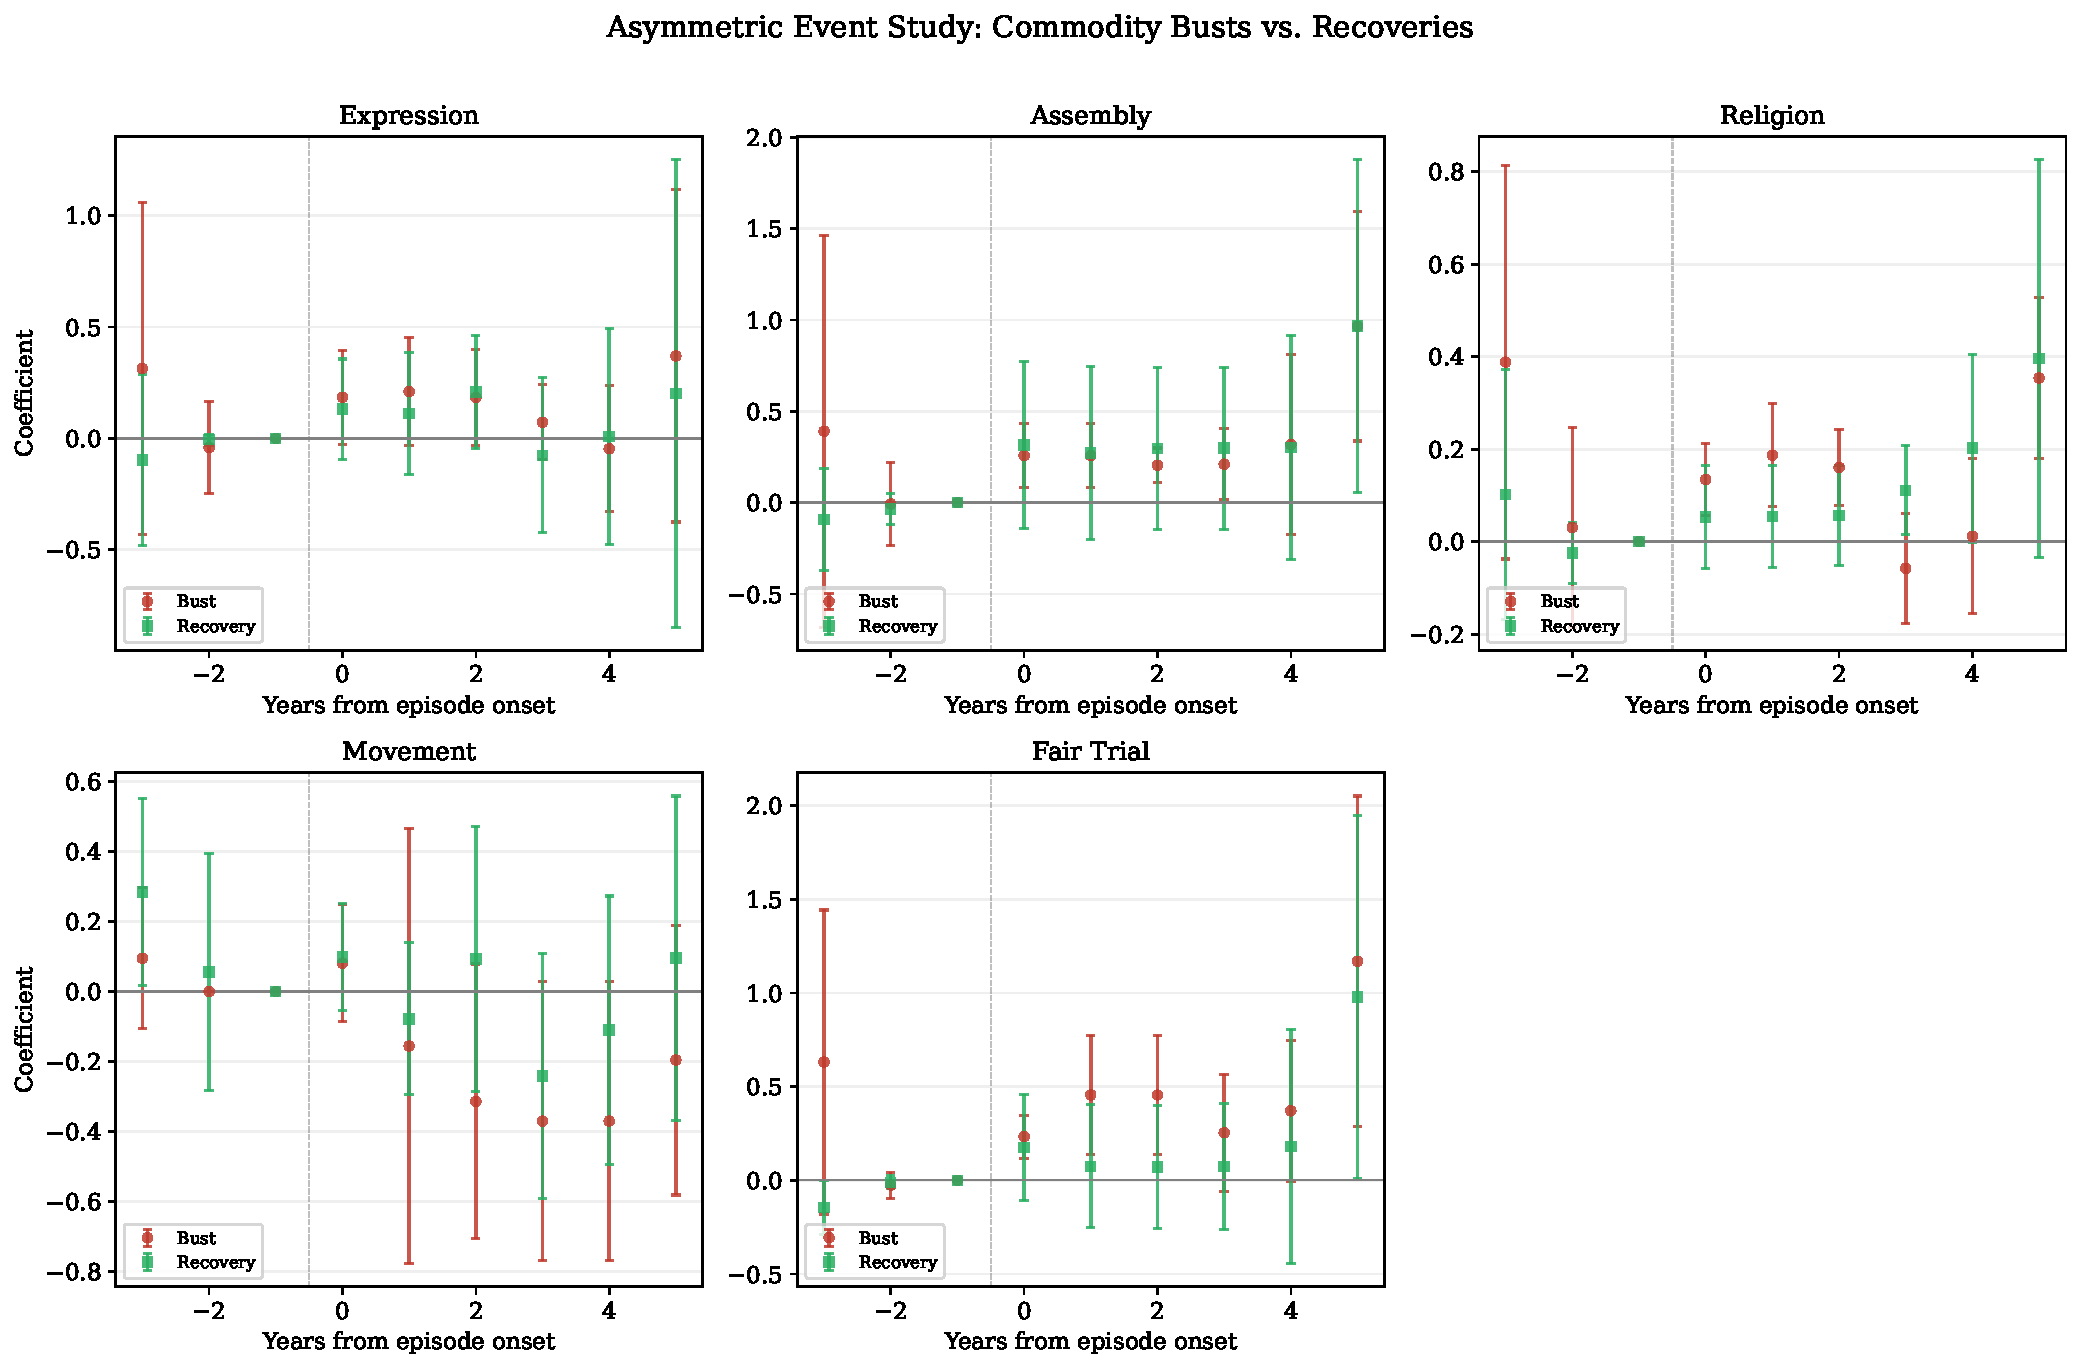
\includegraphics[width=\textwidth]{figures/fig1_asymmetric_event_study.pdf}
\caption{Asymmetric Event Study: Commodity Busts (red) vs. Recoveries (green). Point estimates with 95\% CI. Reference: $t = -1$. All pre-trend $F$-tests: $p > 0.19$.}
\label{fig:event_study}
\end{figure}

\subsection{Symmetry Test}

Table~\ref{tab:symmetry} reports the symmetry test. The null of symmetric effects is rejected for four of five liberties. However, this asymmetry does not uniformly support a ratchet pattern. For assembly, religion, and fair trial, both bust and recovery event-study averages are \textit{positive}, indicating asymmetric improvement trajectories rather than deterioration-without-recovery. Only freedom of movement shows a negative bust average ($-0.220$) with near-zero recovery ($-0.024$), but this result is confounded by COVID-19 restrictions (see Section~\ref{sec:robustness}).

\begin{table}[htbp]
\centering
\caption{Ratchet Test: Symmetry of Bust and Recovery Effects}
\label{tab:symmetry}
\begin{tabular}{lccccc}
\toprule
Liberty & Bust avg. & Recovery avg. & Asymmetry & z-stat & p(symmetry) \\
\midrule
  Expression & 0.1625 & 0.0974 & 0.2599 & 1.949 & 0.051 \\
  Assembly & 0.3688 & 0.4082 & 0.7770 & 5.483 & 0.000 \\
  Religion & 0.1317 & 0.1457 & 0.2774 & 5.370 & 0.000 \\
  Movement & -0.2204 & -0.0235 & -0.2439 & -2.181 & 0.029 \\
  Fair Trial & 0.4891 & 0.2591 & 0.7482 & 5.105 & 0.000 \\
\midrule
\multicolumn{6}{l}{\footnotesize H$_0$: bust effect $=$ $-$recovery effect (symmetry).} \\
\bottomrule
\end{tabular}
\end{table}

\begin{figure}[H]
\centering
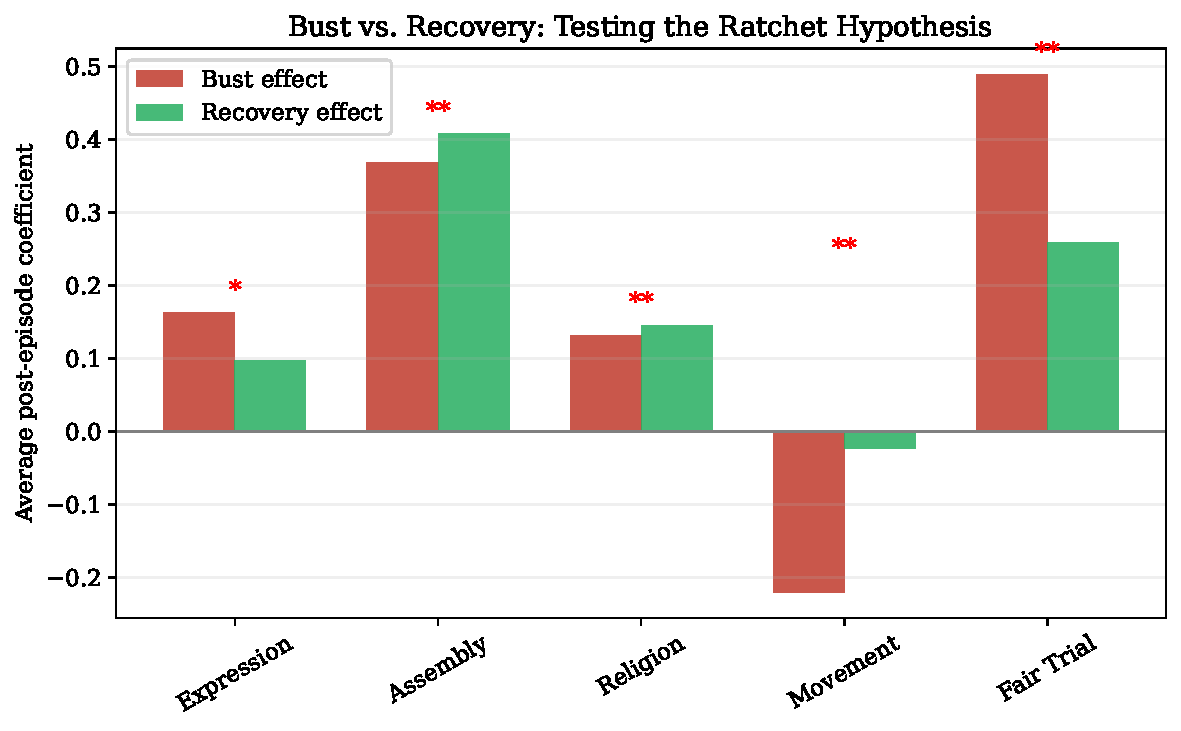
\includegraphics[width=0.8\textwidth]{figures/fig2_symmetry_test.pdf}
\caption{Bust vs. Recovery Effects by Civil Liberty Dimension.}
\label{fig:symmetry}
\end{figure}

\section{Robustness}\label{sec:robustness}

\subsection{COVID-19 Exclusion}

Freedom of movement was identified as the only liberty exhibiting a potential ratchet pattern. However, including 2020--2024 data introduces COVID-19 emergency movement restrictions as a confounder. Excluding 2020--2021, the TWFE bust effect on movement becomes $+0.034$ ($p = 0.705$), eliminating the apparent ratchet. Fair trial rights remain significant at the 10\% level ($\beta = -0.189$, $p = 0.063$), demonstrating robustness to the COVID-era sample restriction.

\subsection{Placebo Timing Tests}

Placebo tests for fair trial (permuting bust dates 999 times) yield $p = 0.389$, and for freedom of movement yield $p = 0.926$. The fair trial placebo $p$-value is above conventional thresholds, consistent with a modest effect that does not dominate the null distribution. The movement placebo confirms that the apparent bust effect is indistinguishable from random timing.

\subsection{Alternative Bust Thresholds}

The fair trial bust effect is robust across thresholds: $-15\%$ ($\beta = -0.154$, $p = 0.066$), $-25\%$ ($\beta = -0.290$, $p = 0.077$), and $-30\%$ ($\beta = -0.149$, $p = 0.020$). The coefficient magnitude increases at stricter thresholds, consistent with a dose-response pattern.

\subsection{Power Analysis}

The minimum detectable effect at 80\% power is 0.21 points (0.22 SD). The fair trial bust effect of $-0.199$ falls just below this threshold, suggesting the study is powered to detect effects of this magnitude but may miss smaller effects in the other four liberties.

\section{Discussion and Conclusion}

This paper provides evidence that commodity busts selectively erode fair trial rights while leaving other civil liberties largely unaffected. The finding is robust to alternative bust thresholds and COVID-era exclusion, though the placebo timing test ($p = 0.389$) suggests the effect, while statistically significant in the parametric test, does not dominate the permutation distribution.

Three lessons emerge. First, disaggregating civil liberties reveals heterogeneity that aggregate indices obscure: the resource curse operates through judicial institutions, not through uniform democratic erosion. Second, the initial finding of a ``ratchet effect'' for freedom of movement illustrates the importance of confounder scrutiny---COVID-19 restrictions generated a pattern indistinguishable from crisis-driven repression. Third, the divergence between bust and recovery dynamics (rejected symmetry in 4/5 liberties) reflects complex institutional trajectories that simple deterioration-recovery narratives cannot capture.

Future research should examine the mechanisms through which commodity busts affect judicial independence, potentially using within-country variation in judicial appointment procedures or court budgets. Microdata from judicial decisions or case backlogs could provide direct evidence of the institutional channel identified here.

\bibliography{references}

\end{document}
